\chapter{Results}\label{sec:results}

This method has been applied in the~real-time planet renderer mentioned in the~introduction on height data of the~whole Earth with the~resolution of 90m (SRTM). Due to the~redundancy of data in the~applied LOD hierarchy, the~size of the~original data was 260GB. With the~maximum error bound set to 5m, the~size of the~compressed data is 7GB, which yields the~compression ratio of 37:1.

For a~comparison, C-BDAM reached the~compression ratio of 64:1 on the~same dataset, but with the~maximum error bound set to 16m. Thanks to the~fact that the~LOD hierarchy of C-BDAM contains no redundancy, the~size of the~original data was just 29GB and the~size of the~compressed data just 870MB. Under such circumstances, only the~comparison in terms of the~compression ratio is relevant.

In Fig.~\ref{fig:result_samples}, you can see a part of a~heightmap compressed by this method, together with the~differences from the~original.

\begin{figure}
	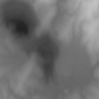
\includegraphics[width=0.4\textwidth]{figures/samp_orig.png}
	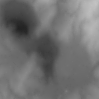
\includegraphics[width=0.4\textwidth]{figures/samp_comp.png}
	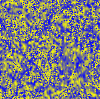
\includegraphics[width=0.4\textwidth]{figures/samp_diff.png}
	\caption{From the~top to the~bottom - the~original terrain, the~same terrain compressed with the~maximum deviation of 5m, the~difference between these~two. The~brighter the~color, the~greater the~value. In the~difference image, the~yellow color means 4.5m, whereas the~blue color means -4.5m.}
	\label{fig:result_samples}
\end{figure}

\newcommand{\incexampl}[1]{\includegraphics[width=0.225\textwidth]{#1}}

\begin{figure}
	\incexampl{figures/dim_64_amp_16_lon_4_horizontal_orig.png}
	\incexampl{figures/dim_64_amp_16_lon_16_horizontal_orig.png}\\\\
	\incexampl{figures/dim_64_amp_16_lon_4_horizontal_out.png}
	\incexampl{figures/dim_64_amp_16_lon_16_horizontal_out.png}\\\\
	\incexampl{figures/dim_64_amp_16_lon_4_horizontal_diff.png}
	\incexampl{figures/dim_64_amp_16_lon_16_horizontal_diff.png}
	\caption{Two synthetic test images of size 64x64, each one containing spiky terrain with the~heights ranging from -16 to 16. On the~left, the~longitude of spikes is 4, on the~right, it is 16. From the~top to the~bottom - the~original, compressed with the~maximum deviation of 5, the~difference between these~two. The~brighter the~color, the~greater the~value. In the~difference image, the~yellow color means 4.5, whereas the~blue color means -4.5.}
	\label{fig:result_wave_samples}
\end{figure}